\newpage
\chapter{Сферические волны}
\par Рассмотрим асимптотику в уравнении
$$  \frac{1}{r^2}\frac{d}{d r} \left(r^2  \frac{d R}{d r} \right) -  \frac{l(l+1)}{r^2} R + \frac{2m}{\hbar^2} (E-U)R =0$$
\par При $r\rightarrow 0$ обычно $\frac{d}{dx} \sim \frac{1}{x}$. И пусть $\lim\limits_{r \to 0}(U\cdot r^2)=0$. Тогда уравнение будет выглядеть следующим образом:
$$ \frac{1}{r^2}\frac{d}{d r} \left(r^2  \frac{d R}{d r} \right) -  \frac{l(l+1)}{r^2} R  =0$$
\par Решение его ищем в виде $R \sim r^s$: $s(s+1)=l(l+1)$, т.е. или $s=l$, или $s=-(l+1)$
\par При $r\rightarrow \infty$ и  $\lim\limits_{r \to \infty}(U)=0$ получим 
$$ \frac{1}{r^2}\frac{d}{d r} \left(r^2  \frac{d R}{d r} \right) -  \frac{l(l+1)}{r^2} R + \frac{2m}{\hbar^2} (E-\cancel{U})R =0$$
\par $E = \frac{\hbar^2}{2m}$. Получается задача о свободной частице с решением в виде плоских волн, спектр непрерывный (к - импульс плоских волн). Проблема в 3D - вырожденный спектр. 
\par Фактически, нам нужно перейти от плоских волн к сферическим. $\Delta \psi + k^2 \psi =0$ - решение есть потенциал сферического источника, при k=0 это $1/r$. Индексы: $k$ - модуль импульса, $l $- момент.
$$R^{\prime \prime}_{kl} + \frac{2}{r}R^\prime _{kl} +\left(k^2 - \frac{l(l+1)}{r^2} \right)R _{kl}=0$$
\par Нормировка $\int^\infty_0 r^\prime R_{k^\prime l}R_{kl}dr=2\pi \delta (k^\prime- k)$. Пусть $l=0$, тогда $R_{k0}= 2 \frac{sin kr}{r}$ (вообще перед $\frac{e^{\pm ikr}}{r}$ может быть любая константа, но именно двойка будет очень удобна). При $l \ne 0$ получим $R_{kl}= r^l \chi_{kl}(r)$. Уравнение на $\chi$:
$$\chi^{\prime \prime}_{kl} + \frac{2(l+1)}{r}\chi^{\prime}_{kl} + k^2 \chi_{kl} =0 $$
\par Продифференцируем его $\frac{\partial}{\partial r}$:
$$\chi^{\prime \prime \prime}_{kl}+ \frac{2(l+1)}{r}\chi^{\prime \prime}_{kl} + \left( k^2 - \frac{2(l+1)}{r^2} \right)\chi^{\prime}_{kl}=0 $$
\par Т.к. $\chi^{\prime}_{kl} = r \chi_{k,l+1}$, то, во-первых,
$$\chi^{\prime \prime \prime}_{kl}+ \frac{2(l+1)}{r}\chi^{\prime }_{k,l+1} +  k^2 \chi_{k,l+1}=0$$
\par И, во-вторых, $\chi_{kl}= \left(\frac{1}{r} \frac{d}{dr} \right)^l \chi_{k0}$. Получим $R_{kl} = (-1)^l 2 \frac{r^l}{k^l} \left(\frac{1}{r} \frac{d}{dr} \right)^l  \frac{sin kr}{r} = \sqrt{\frac{2 \pi k}{r}} J_{l+1/2}(kr)$ или же $R_{kl} = 2 k j_l(kr)$, где $j_l(kr)$ - сферическая функция Бесселя (или  функция Бесселя 2 рода).

\par \begin{wrapfigure}[5]{c}{1\linewidth} 
\vspace{-2ex}
\centering
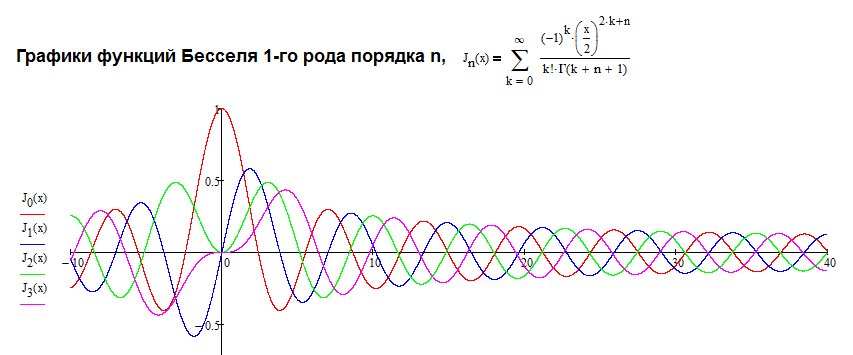
\includegraphics[width=1\linewidth]{pictures/28.1.png}
\caption{Функции Бесселя 1 рода}
\end{wrapfigure}

\par \begin{wrapfigure}[10]{r}{0.4\linewidth} 
\vspace{-2ex}
\centering
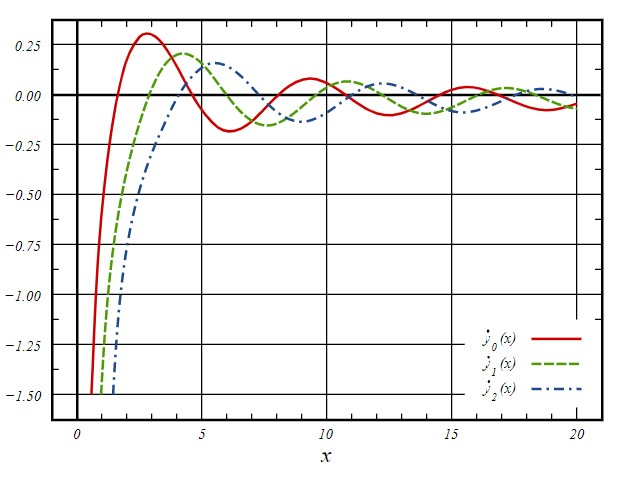
\includegraphics[width=1\linewidth]{pictures/28.2.jpg}
\caption{Функции Бесселя 2 рода}
\end{wrapfigure}
\par Асимптотики решения: $r \rightarrow \infty$ $R_{kl}\rightarrow \frac{2}{r} sin (kr- \pi l/2) $, при $ r \rightarrow 0$ $R_{kl}\rightarrow \frac{2k^{l+1}}{(2l+1)!!} r^l $.
\par $z = r cos \theta$: 
$$e^{ikz}=\sum^\infty_{l=0}(-i)^l(2l+1)P_l (cos\theta) \frac{r}{k}^l \left(\frac{1}{r} \frac{d}{dr} \right)^l  \frac{sin kr}{r}$$
\par $\forall \vec{k}$ можем выбрать ось $Oz$ и написать такое разложение, поэтому оно самого общего вида.